\subsection{Class Diagram}


The class diagram contains a selection of the classes used to handle books and users within the Bookly web application. It includes two main servlets: the \textit{BookServlet}, which manages the book resource, and the \textit{UserServlet}, which handles user-related functionality such as login and registration. Each servlet extends the \textit{AbstractDatabaseServlet}, which provides shared logic for acquiring a database connection from the connection pool.
\medskip

The \textit{BookServlet} implements the \texttt{doGet} method to retrieve either a list of all books or the details of a specific book, depending on the URI pattern. These operations are delegated to the DAO classes \textit{GetAllBooksDAO} and \textit{GetBookByIdDAO}, both of which extend the \textit{AbstractDAO\textless Book\textgreater} class and implement the \texttt{doAccess()} method to execute SQL statements and return data as \textit{Book} objects.

\medskip

The \textit{UserServlet} implements both \texttt{doGet} and \texttt{doPost} methods to support login and registration functionality. Before interacting with the database, it uses the \textit{LoginServices} and \textit{RegisterServices} classes to validate input. If validation succeeds, it calls either \textit{LoginUserDAO} or \textit{RegisterUserDAO}, depending on the operation. These DAO classes extend \textit{AbstractDAO\textless User\textgreater} and are responsible for retrieving or inserting user data, including profile images if provided.
\medskip

The \textit{User} and \textit{Book} classes represent the core entities in the application. Each class contains multiple fields and standard accessors. The \textit{User} class also references additional entities such as \textit{Order}, \textit{Cart}, and \textit{Wishlist}, which are not expanded in this diagram. Both the \textit{User} and \textit{Book} classes contain an \textit{Image} field to represent profile or cover images using the \textit{Image} class.
\medskip

All DAO classes inherit from the generic abstract class \textit{AbstractDAO\textless T\textgreater}, which manages consistent database access and exception handling. Each subclass implements the \texttt{doAccess()} method to define specific SQL logic. The \textit{AbstractDAO} class also includes mechanisms to control access and return output parameters.

This class diagram focuses on the core application logic behind user authentication, registration, and book browsing functionality. It reflects the architectural layering of the application, with clear separation between controllers (servlets), data access logic (DAOs), business validation (services), and data representation (resources).
\medskip

\begin{figure}[h]
    \centering
    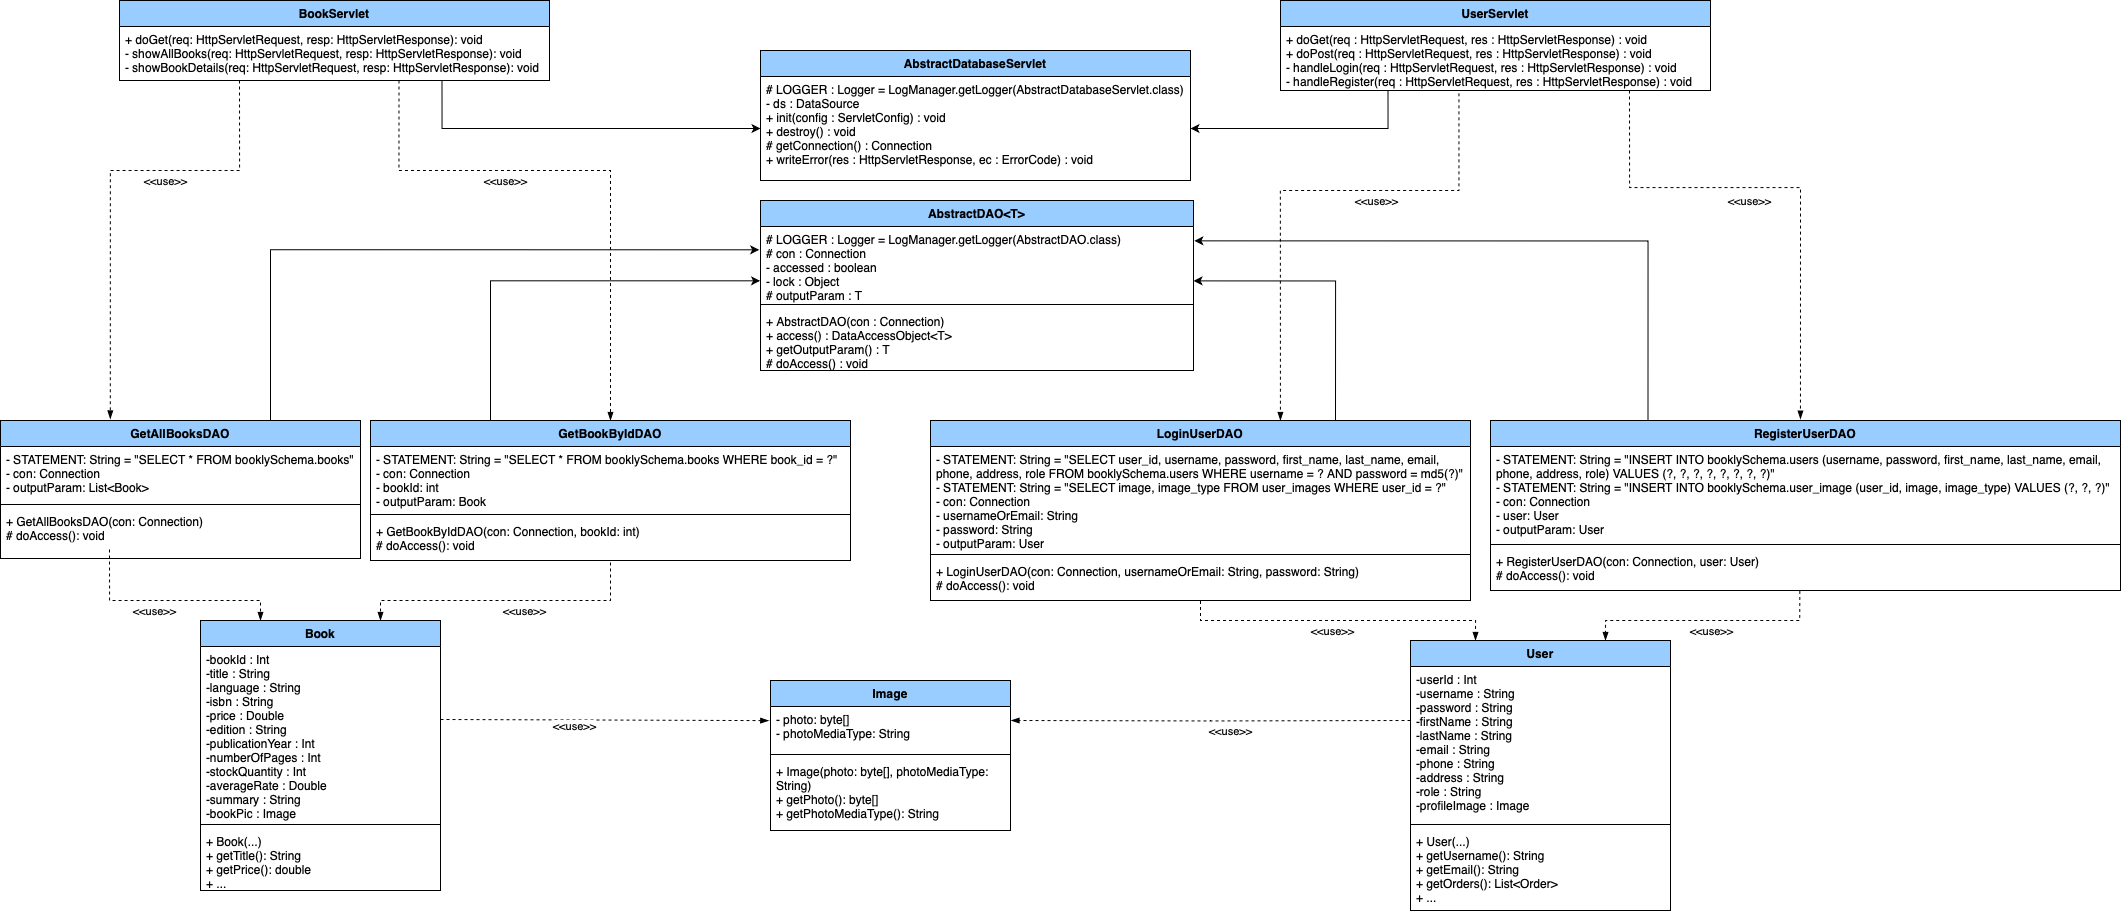
\includegraphics[width=\textwidth]{HW1Report/photos/ClassDiagram.png}
    \caption{Class diagram of the Bookly web application}
    \label{fig:classdiagram}
\end{figure}

\begin{figure}[h]
    \centering
    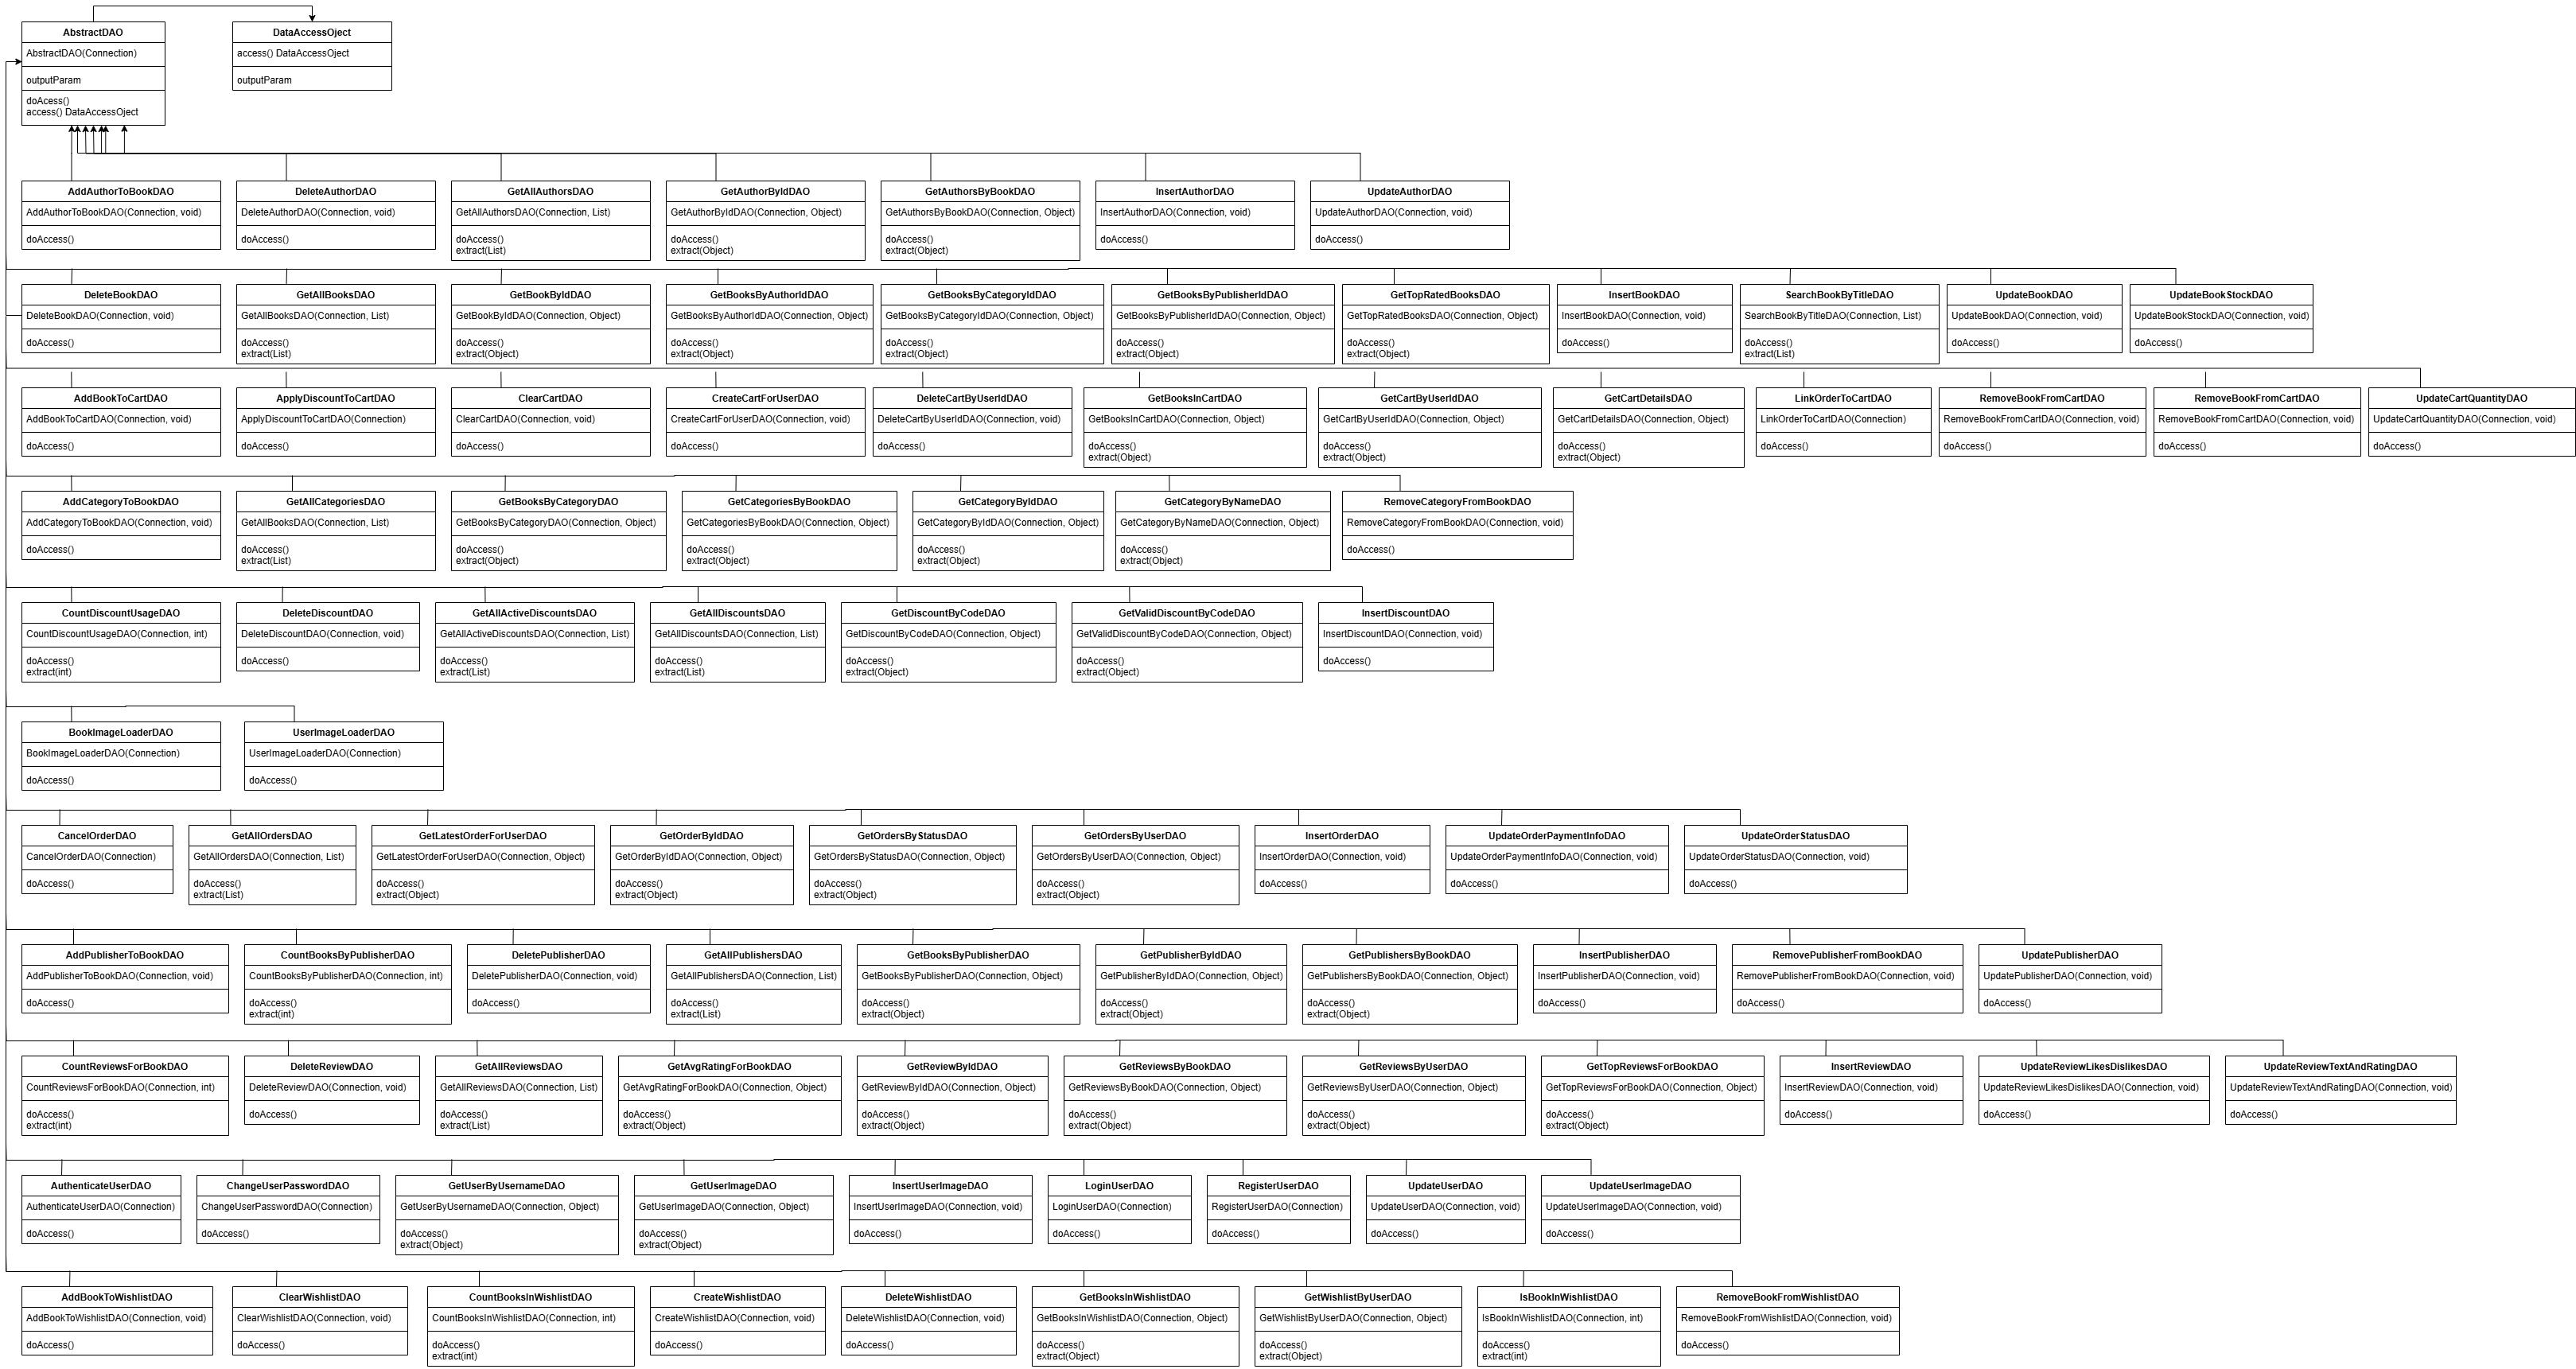
\includegraphics[width=\textwidth]{HW1Report/photos/dao-class-diagram.png}
    \caption{DAO Classes diagram of the Bookly web application}
    \label{fig:daoclassdiagram}
\end{figure}